

\tikzset{every picture/.style={line width=0.75pt}} %set default line width to 0.75pt        

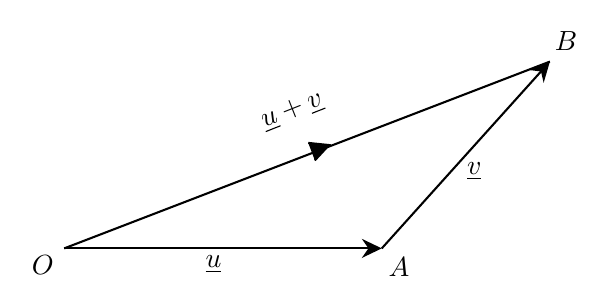
\begin{tikzpicture}[x=0.75pt,y=0.75pt,yscale=-0.9,xscale=0.9]
%uncomment if require: \path (0,300); %set diagram left start at 0, and has height of 300

%Straight Lines [id:da3683399638260374] 
\draw    (200,180) -- (367,180) ;
\draw [shift={(370,180)}, rotate = 180] [fill={rgb, 255:red, 0; green, 0; blue, 0 }  ][line width=0.08]  [draw opacity=0] (10.72,-5.15) -- (0,0) -- (10.72,5.15) -- (7.12,0) -- cycle    ;
%Straight Lines [id:da012426198552259127] 
\draw    (370,180) -- (457.99,82.23) ;
\draw [shift={(460,80)}, rotate = 491.99] [fill={rgb, 255:red, 0; green, 0; blue, 0 }  ][line width=0.08]  [draw opacity=0] (10.72,-5.15) -- (0,0) -- (10.72,5.15) -- (7.12,0) -- cycle    ;
%Straight Lines [id:da507431700036358] 
\draw    (200,180) -- (460,80) ;
\draw  [fill={rgb, 255:red, 0; green, 0; blue, 0 }  ,fill opacity=1 ] (330.64,123.53) -- (341.77,124.68) -- (334.18,132.89) ;

% Text Node
\draw (181,182.4) node [anchor=north west][inner sep=0.75pt]    {$O$};
% Text Node
\draw (372,183.4) node [anchor=north west][inner sep=0.75pt]    {$A$};
% Text Node
\draw (461,62.4) node [anchor=north west][inner sep=0.75pt]    {$B$};
% Text Node
\draw (274,182.4) node [anchor=north west][inner sep=0.75pt]    {$\underline{u}$};
% Text Node
\draw (301.81,106.57) node [anchor=north west][inner sep=0.75pt]  [rotate=-338.43]  {$\underline{u} +\underline{v}$};
% Text Node
\draw (414,132.4) node [anchor=north west][inner sep=0.75pt]    {$\underline{v}$};


\end{tikzpicture}